% !Mode:: "TeX:UTF-8:Main"
\documentclass[aspectratio=169]{beamer}
\usepackage{tikz}
\usetikzlibrary{tikzlings,ducks}
\usetikzlibrary{calc}
\setbeamertemplate{navigation symbols}{}
\setbeamertemplate{background canvas}{\makebox[\paperwidth][l]{%
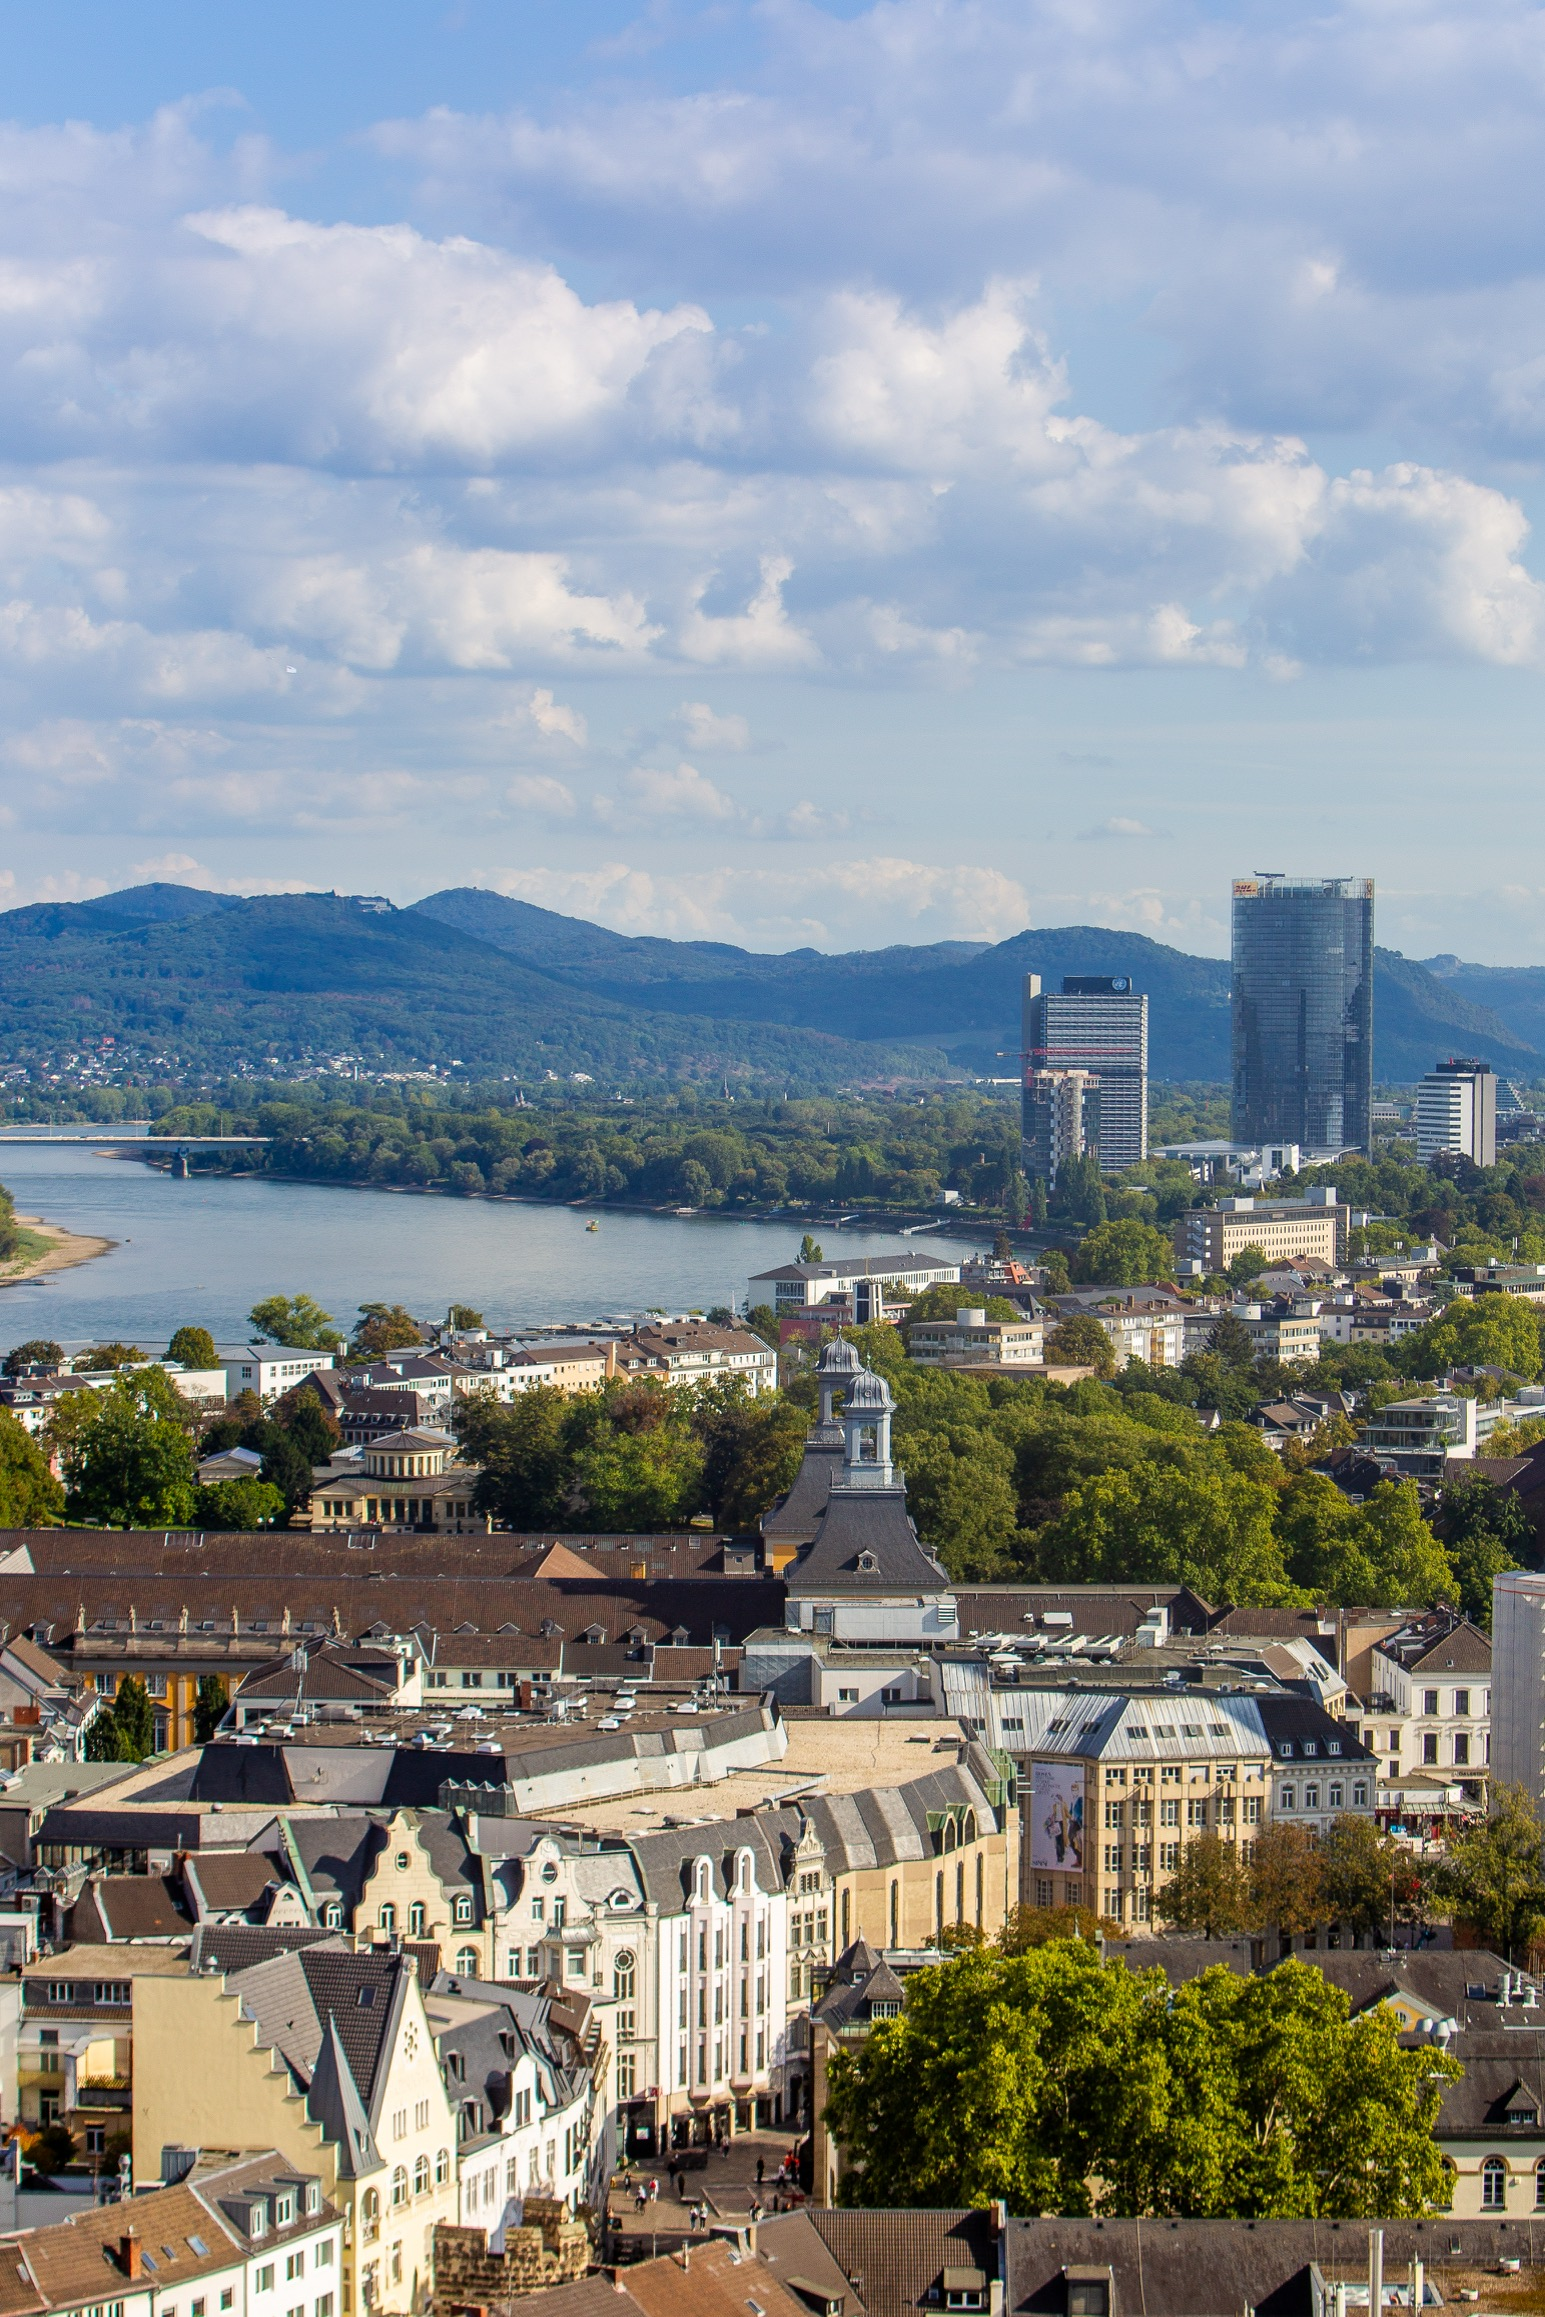
\includegraphics[trim=0cm 12cm 0cm 10cm,height=\paperheight]{bonn}}}

% trick taken from https://topanswers.xyz/tex?q=1989
\tikzset{
    use page relative coordinates/.style={
        shift={(current page.south west)},
        x={(current page.south east)},
        y={(current page.north west)}
    },
}
\usepackage{graphicx,bearwear}
\begin{document}
\begin{frame}
\hspace*{\dimexpr-1in+\oddsidemargin}%
\begin{tikzpicture}[remember picture] \path[use as 
bounding box](0,0)--(\textwidth,\textheight-14.7pt); 

\node[anchor=south west,font=\large] at (0.85\textwidth, -0.15\textheight)
 {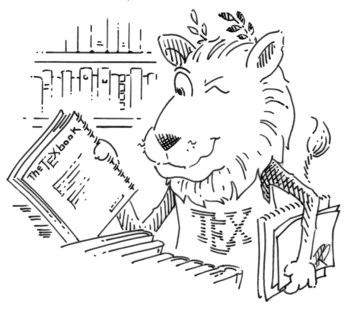
\includegraphics[width=0.5\textwidth]{ctan-lion}};

\node[anchor=base,font=\Large\bfseries] at (1.1\textwidth, 0.75\textheight)
 {\begin{tabular}{c}
   \TeX~Users~Group \\ 
   Conference\\
   14.--16.~JULY 2023\\
   Bonn, Germany
  \end{tabular}};
  

\path[] (4cm+\fpeval{\the\value{page}/600*2.5}cm,
         0.4\textheight-\fpeval{\the\value{page}/600*0.5}cm) 
         pic[xscale=-1,scale=\fpeval{0.2+\the\value{page}/3000}]{duck};

\begin{scope}
\path%[draw,red]%
[clip] (0.4\textwidth,\textheight)--(0.65\textwidth,\textheight)--++ 
(0,-0.38\textheight-10.7pt)--++(-0.15\textwidth,-1.5mm)--++(-0.1\textwidth,2.5mm)--cycle; 
  
\begin{scope}[shift={($(0.5\textwidth,0.25\textheight)+(0,\fpeval{\the\value{page}/600*0.3}\textheight)$)}]

\bear[signpost={\begin{tabular}{c}TUG\\ 2023\end{tabular}},
signcolour= brown!50!black,
signback=green!40!black]\bearwear[body deco=
{\node[fill=white,inner sep=0.4pt] at ([yshift=0mm]beartummy)
  {
\includegraphics[trim=0cm 25pt 0pt 0pt,clip,width=0.6cm]{kussmund}};
}]


\end{scope}
\end{scope}

\begin{scope}[use page relative coordinates]
\node[font=\tiny,anchor=east,rotate=90] at (.01,.999) {Background image: Copyright Bundesstadt Bonn};
\end{scope}

\end{tikzpicture}
\pause[600]
\end{frame}
\end{document}
https://m.youtube.com/watch?v=O7Iu5Vyo1us 0.0--030 
